%%
%% licence       kaneton licence
%%
%% project       kaneton
%%
%% file          /home/buckman/kaneton/view/books/assignments-k1/k1.tex
%%
%% created       matthieu bucchianeri   [tue feb  7 11:49:56 2006]
%% updated       matthieu bucchianeri   [sun feb 11 22:54:06 2007]
%%

%
% k1
%

\chapter{k1: memory management}

%
% informations
%

\begin{tabular}{p{7cm}l}
  Duration: & 2 weeks \\
  File name: & {\em login\_x}-k1.tar.bz2 \\
  In charge: & Julian Pidancet \& Elie Bleton\\
  Newsgroup: & epita.cours.kaneton \\
  Languages: & C \\
  Students per group: & 2 \\
\end{tabular}

\section{Abstract}

k1 project consists in developing a large part of the kaneton memory management. Using all the concepts learned in class, you will have to implement:

\begin{enumerate}
\item
  {\bf The segment manager}\\
  Manage physical memory
\item
  {\bf The region manager}\\
  Manage virtual memory
\item
  {\bf The map manager}\\
  Assume the mapping between physical and virtual memory.\\
\end{enumerate}

This part of the kaneton project introduces important notions around the
kaneton design.

For the first time, you will have to write kaneton managers. This point is
very important since one of the fundamental concepts of kaneton microkernel
is to be subdivided into managers.

The kaneton microkernel was also designed to be ported on many
architectures. It uses specific macro functions to import and call
architecture-dependent routines. You will also have
to understand this concept and to study how it is implemented in the
kaneton microkernel. This feature is heavily used in the region manager since
most of its job is actually done in the architecture-dependent code.

%
% Segment manager
%

\newpage

\section{Segment manager}

\subsection*{Overview}
The segment manager provides a complete interface to manipulate physical
memory areas called {\em segments}. It is called everytime the kernel
needs to allocate, modify or free a physical memory area.\\

In other words, the segment manager interface provides:
\begin{itemize}
\item a physical memory allocator
\item physical memory read/write operations
\item a way to set physical memory areas attributes (size, permissions, \ldots)
\end{itemize}

\textbf{Beware:} Kaneton's segments doesn't have anything to do with Intel's segmentation mechanism.
In kaneton, segments are \textit{just} an abstraction for physical memory.

\subsection*{Assignments}
In k1, you will write the entire segment manager. That includes the
machine-independent part of the manager, as well as the machine-dependent
code.\\

The architecture-dependent code must always be invoked using the kaneton
internal portability facilities.\\
\\
Your segment manager must be compliant to the kaneton segment manager
interface as described below.

\subsection*{Files}

{\color{filerefcolor} \textbf{machine-independent}}
\begin{itemize}
\item kaneton/core/segment/segment.c
\item kaneton/core/segment/segment-fit.c
\end{itemize}

{\color{filerefcolor} \textbf{machine-dependent}}
\begin{itemize}
\item kaneton/machine/architecture/ia32/generic/segment.c
\item kaneton/machine/glue/ibm-pc.ia32/educational/segment.c
\end{itemize}

\subsection*{Required implementation}
You \textit{must} implement these functions. We give you their prototypes
and a small description of what they are expected to do.
\textit{All these functions are machine-independant EXCEPTED segment\_read, segment\_write and segment\_copy.}

\function{segment\_reserve}{(i\_as \argument{as},
  t\_psize \argument{size},
  t\_perms \argument{perms},
  i\_segment* \argument{id})}
{
  This function reserves in the address space
  \argument{as} a segment with specified properties.
  \newline
  This function calls the physical memory allocator, implemented
  in function \emph{segment\_space} (see segment-fit.c).
  The identifier of the reserved segment is returned in \argument{id}.
}

\function{segment\_first\_fit}{(o\_as* \argument{as},
  t\_psize \argument{size},
  t\_paddr* \argument{address})}
{
  This function allocates for the address space \argument{as} a
  contiguous space of size \argument{size} in physical
  memory. The address of the beginning of the allocated block is
  returned in \argument{address}.
  \newline
  We \textbf{require} you to implement \textit{at least}
  segment\_first\_fit !
  \newline
  If you want to implement any other method, see segment\_space
  to see how you can plug-in.
}

\function{segment\_release}{(i\_segment \argument{id})}
{
  This function releases the segment \argument{id}.
}


\function{segment\_inject}{(i\_as \argument{as},
  o\_segment* \argument{o},
  i\_segment* \argument  printf("Attempting");{segid})}
{
  This function injects a pre-allocated segment in the
  address space \argument{as}. It means that no physical
  memory is allocated, the \argument{o} structure is
  trusted to be correctly filled.
}

\function{segment\_get}{(i\_segment \argument{segid},
  o\_segment** \argument{o})}
{
  This function retrieves a segment object \argument{o} given its identifier
  \argument{segid}.
}

\function{segment\_flush}{(i\_as \argument{as})}
{
  This function removes every segment that belongs to
  the address space \argument{as} and releases the
  physical memory associated.
}

\function{segment\_clone}{(i\_as \argument{as},
  i\_segment \argument{old},
  i\_segment* \argument{new})}
{
  This function clones a segment which will then belong to
  the address space object \argument{as}.

  Cloning a segment means reserving a new segment with the
  exact same properties. Then the content is also copied.
}

\function{segment\_read}{(i\_segment \argument{id},
  t\_paddr \argument{offset},
  void* \argument{buffer},
  t\_psize \argument{size})}
{
  This function reads \argument{size} bytes at offset
  \argument{offset} from the segment \argument{id}. \newline
  \textbf{This function requires a working region module !}
}

\function{segment\_write}{(i\_segment \argument{id},
  t\_paddr \argument{offset},
  const void* \argument{buffer},
  t\_psize \argument{size})}
{
  This function write the data of \argument{buffer} into the
  segment \argument{id}. \newline
  \textbf{This function requires a working region module !}
}

\function{segment\_copy}{(i\_segment \argument{dst},
  t\_paddr \argument{offd},
  i\_segment \argument{src},
  t\_paddr \argument{offs},
  t\_psize \argument{size})}
{
  This function copies data from the segment \argument{src} to
  the segment \argument{dst}. \newline
  \textbf{This function requires a working region module !}
}

\function{segment\_perms}{(i\_segment \argument{id},
  t\_perms \argument{perms})}
{
  This function changes the permissions of the segment \argument{id}.
}


%
% region manager
%

\newpage

\section{Region manager}
\subsection*{Overview}
The region manager provides a complete interface to manipulate virtual memory
areas called {\em regions}. It is used to reserve virtual memory and to map it
on segments.\\
\\
The region manager thus provides:

\begin{itemize}
\item a virtual memory allocator
\item virtual memory mapping routines\\
\end{itemize}

{\em Warning:}\\
the region manager always deals with existing valid segments. In
other terms, it never reserves, releases or modifies a segment to fit the mapping
needs. Such an initiative is handled by the map manager.

\subsection*{Assignments}
In k1, you will write the machine-dependent code of the kaneton region manager.
This code implements an interface between the machine-independent manager, and
the specific needs of the IA-32 architecture.
\\ \\
You are also asked to respect the given interface and to use the provided
libarch low-level functions. You are strongly advised to check the machine-independent code to
understand how machine-dependant code will be called.
\\ \\
The following functions are given (except \emph{region\_space}, very similar to \emph{segment\_space}), but you must write the code in
the architecture-dependent side of the manager.

\subsection*{Files}
{\color{filerefcolor} \textbf{machine-independent}}
\begin{itemize}
\item kaneton/core/region/region.c (\textbf{strongly advised reading})
\item kaneton/core/region/region-fit.c (for region\_first\_fit)
\end{itemize}

{\color{filerefcolor} \textbf{machine-dependent or architecture-dependant}}
\begin{itemize}
\item kaneton/machine/glue/ibm-pc.ia32/educational/region.c
\item kaneton/machine/glue/ibm-pc.ia32/educational/include/region.h
\end{itemize}

\newpage
\subsection*{Required implementation}

\function{region\_first\_fit}{(o\_as* \argument{as},
  t\_vsize \argument{vsize},
  t\_vaddr* \argument{address})}
{
  Refer to \textit{segment\_first\_fit} to picture out what this does. \newline
  A significant difference is that region\_first\_fit works with regions instead of segments.
}

\function{glue\_region\_reserve}{(i\_as \argument{as},
  i\_segment \argument{segment},
  t\_paddr \argument{offset},
  t\_opts \argument{opts},
  t\_vaddr \argument{address},
  t\_vsize \argument{size},
  i\_region* \argument{id})}
{
  This function reserves a region with specified properties
  into the address space \argument{as}. This region maps the
  segment given by \argument{segment}. The identifier of the reserved
  region is returned in \argument{id}.
  \newline
  Values for \argument{opts} can be:
  \begin{itemize}
  \item {REGION\_OPT\_NONE}: no options
  \item {REGION\_OPT\_FORCE}: forces the region to be reserved at address \argument{address}. Otherwise, uses \emph{region\_space} to allocate the region.
  \item {REGION\_OPT\_USER}: set the region addressable in both user and kernel mode
  \item {REGION\_OPT\_PRIVILEGED}: set the region to be addressable in kernel mode only
  \item {REGION\_OPT\_LOCAL}: set the region to be local to the address space
  \item {REGION\_OPT\_GLOBAL}: set the region to be global over all address spaces
  \end{itemize}

  The \argument{offset} indicates where to start mapping
  physical address. For example, reserving two regions on a
  single segment is allowed.
  \begin{center}
    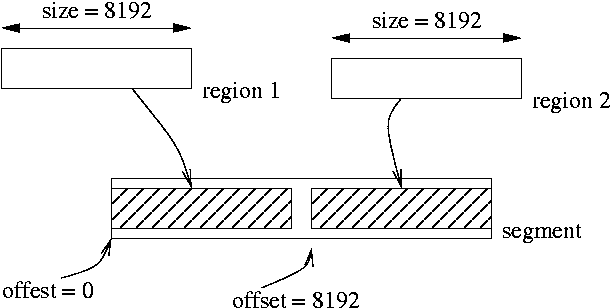
\includegraphics[width=0.4\linewidth]{figures/offset}
  \end{center}

  This function is \textbf{really long}, even if you split it. So split it \textbf{a lot} and \textbf{wisely}.
}

\function{glue\_region\_release}{(i\_as \argument{as},
  i\_region \argument{id})}
{
  This function releases the region \argument{id} that
  belongs to the address space object \argument{as}. Be
  careful, releasing a region does not mean releasing the
  associated segment.
}

%
% Map manager
%

\newpage

\section{Map manager}

\subsection*{Overview}
The map manager implements a high-level interface to manipulate memory mappings.
It directly depends on both segment and region managers.\\
\\
For example, reserving a map consists in the two following steps:
\begin{itemize}
\item ask the segment manager to reserve physical memory.
\item ask the region manager to map this memory on virtual addresses.\\
\end{itemize}

{\em Note:}\\
As the map manager's role is to delegate its tasks to lower managers, it does
not require to implement a machine-dependent interface.

\subsection*{Assignments}
In k1, you will write the whole map manager. This manager will use the segment
and region manager you implemented sooner.\\
\\
As usual, your map manager must conform to the kaneton map manager interface as
described as follow.\\
\\
In addition, you will have to provide a wrapper to classical
\emph{mmap} and \emph{munmap} functions.

\subsection*{Files}

\begin{tabular}{| l | l |}
  \hline
  machine-independent & {\em kaneton/core/map/map.c}\\\hline
\end{tabular}

\subsection*{Required Implementation}

\function{map\_reserve}{(i\_as \argument{as},
  t\_opts \argument{opts},
  t\_vsize \argument{size},
  t\_perms \argument{perms},
  t\_vaddr* \argument{address})}
{
  This function reserves some physical memory and map it into
  the address space \argument{as}.  The segment will have the
  size \argument{size} with the permissions \argument{perms}
  while the region will map the whole segment.

  The virtual address is returned in \argument{address}. The
  values for \argument{opts} can be:
  \begin{itemize}
  \item {MAP\_OPT\_NONE}: no option is specified
  \item {MAP\_OPT\_FORCE}: forces the memory to be allocated at virtual address \argument{address}
  \item {MAP\_OPT\_USER}: set permissions for both user and kernel
  \item {MAP\_OPT\_PRIVILEGED}: set permissions for kernel only
  \end{itemize}
}

\function{map\_release}{(i\_as \argument{as},
  t\_vaddr \argument{address})}
{
  This function releases a previously reserved map, this
  includes releasing both virtual and physical memory.
}

%
% advanced topics
%

\newpage

\section{Bonuses}

kaneton microkernel is first of all a pedagogical project which do not ains at being
optimized. That is why, when nothing is specified, you always will implement the simplest
algorithms.\\
\\
Nevertheless, we will always encourage students who want to write additional bonuses, as far as they respect the following rules:
\begin{enumerate}
\item Bonuses will be evaluated only if a basic implementation is actually working.
\item Bonuses must be accepted \textbf{prior to the implementation} by the kaneton team.
\end{enumerate}

Bonuses ideas:
\begin{itemize}
\item Buddy system
\item Slab allocator
\end{itemize}
